
\section*{Welcome Address}\addcontentsline{toc}{section}{Welcome Address}

It is our great pleasure to welcome you to the 2019 meeting of the Society for Music Perception and Cognition, hosted by New York University.  It's an exciting time for NYU, which has recently seen the development of new interdisciplinary endeavors in music and science.  The Music and Audio Research Laboratory (MARL), which originated as the research arm of the Music Technology Program at NYU and has music cognition as one of its focus areas, is now an official Center at NYU. This past spring, NYU and the Max Planck Institute for Empirical Aesthetics in Frankfurt established the Max Planck-NYU Center for Language, Music and Emotion (CLaME).  We're thrilled to be able to host SMPC 2019 at NYU and hope that both SMPC and the university will benefit from the potential research cross-pollination and collaboration opportunities that will arise from the conference events.
 
We had a record number of submissions this year, resulting in 156 talks, 164 posters, and 7 symposia on the program.  We are also excited to have a large international contingent, hailing from around the world.  Back by popular demand are the faculty-student lunches, as well as two early career panels.  There will also be a panel featuring journal editors and a seminar on applying to grad school.  We have two big social events planned: our opening reception on August 5 and a Circle Line dinner cruise around Manhattan on August 6.  As you experience the conference, please feel free to add your comments and reflections on the SMPC conference Facebook page and on Instagram and Twitter (\#smpc2019).
 
You will also notice a shorter format for both the conference itself and the paper presentations compared to recent years. In order to make it financially accessible for as many attendees as possible, we limited the conference events to three days and secured dorm housing to help reduce travel costs. We shortened the talk time slots to 15 minutes to allow us to remain inclusive in the more limited time frame. We also opted for a dinner cruise instead of a traditional banquet to provide an opportunity for SMPC attendees to experience New York City while connecting with each other in a more open social format. 
 
This conference would not be possible without the help of the many colleagues and administrative staff who contributed to all aspects of the conference.  We are able to present a diverse and extensive program thanks to our 88-person scientific committee and meta-reviewers, whose contributions made it possible to assign three reviews per submission.  Special thanks also to the administrative and technical staff in the Department of Music and Performing Arts Professions, the Steinhardt School, and the Kimmel Center, whose time and dedication have been crucial to the success of this conference.
\\
\\
Sincerely,
\\
\indent Mary Farbood and Johanna Devaney, Conference Chairs

Peter Martens, Program Chair

Finn Upham, Publicity and Publication Chair

\begin{figure}[H]
\centering
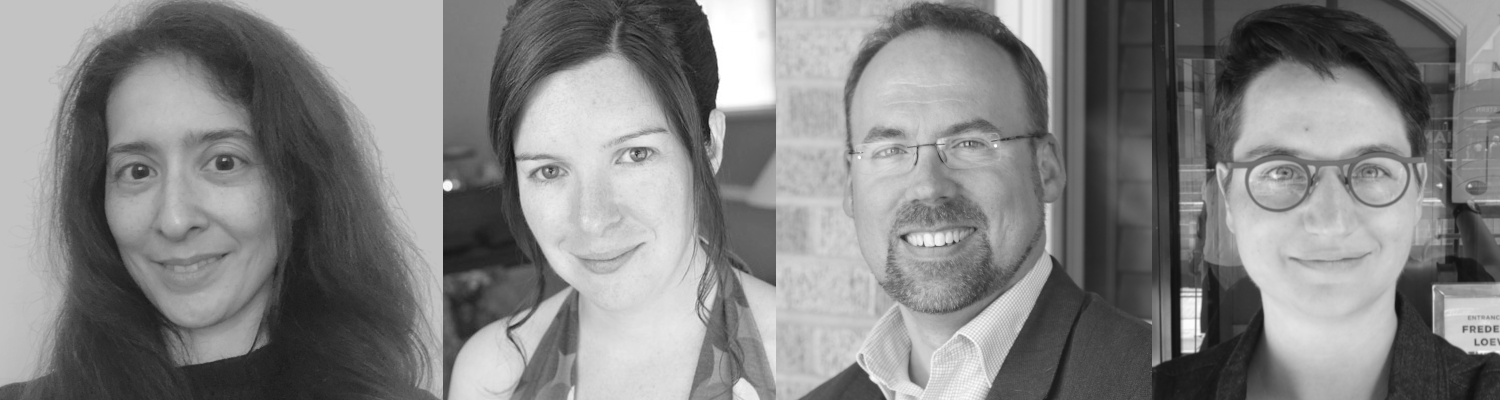
\includegraphics[width=1\linewidth]{images/Chairs_photo_2.png}
\end{figure}
